\documentclass[nofonts]{ctexart}

% 设置中文字体
\setCJKmainfont{WenQuanYi Micro Hei Mono}
\setCJKsansfont{WenQuanYi Micro Hei Mono}
\setCJKmonofont{WenQuanYi Micro Hei Mono}

% 设置英文字体
\setmainfont{Times New Roman}
\setsansfont{WenQuanYi Micro Hei Mono}
\setmonofont{FreeMono}

\usepackage{graphicx}
\usepackage{caption}

\begin{document}
\begin{figure}
	\centering
	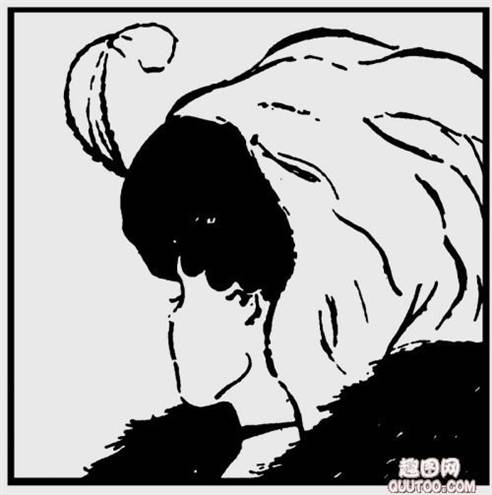
\includegraphics[width=0.4\textwidth]{lady.jpg}
	\qquad
	\parbox[b]{0.4\textwidth}{这只狮子是由画师 Duane Bibby 专门为著名的
		\TeX 发行版 TeXLive 绘制的作品. 狮子是 \TeX 系统的吉祥物, Duane
		Bibby 创作了大量有关 \TeX 狮子的插图, 如高德纳的
		\textit{The System} 两书中的狮子插图, 就是由 Duane Bibby 创作的.
	}
	\caption{\TeX 狮子}\label{fig:textlivelion}
\end{figure}
\end{document}
